% Runtime View — arc42 §6, Scenario 1: a full aggregate() call.
% Notation: UML 2.5 activity diagram (OMG UML 2.5.1, clause 15 "Activities").
%
% Why TikZ: every node is placed by hand in millimetres and every long edge is
% routed down an explicitly chosen free lane, so no connector can be pushed
% through a box. Font sizes are real points (\footnotesize = 8 pt at a 10 pt
% base), so the print budget holds BY CONSTRUCTION.
%
% ── PRINT TARGET ──────────────────────────────────────────────────────────
% "AutoRecovery save of ETHOS.docx" is US Letter (12240 x 15840 twips) with
% 1 inch margins, so the text column is 165.1 x 228.6 mm and every figure in it
% is placed at the full 165 mm width (wp:extent cx="5943600" EMU). What matters
% is therefore the ASPECT RATIO, not the raw size: at 165 mm wide the drawing
% renders 165 * (h/w) mm tall, and that has to leave room for a caption. Budget:
% h/w <= 1.24, i.e. <= 205 mm tall. This file lands at 1.21 (199 mm at 165 wide).
%
% ── LAYOUT ────────────────────────────────────────────────────────────────
% THREE columns, not two. Two columns forced 14 nodes into one 185 mm column,
% which left only 2 mm between the boxes at the bottom — not enough for an
% arrow to be visible. Three columns of 9-10 nodes give every edge >= 4.5 mm
% and every diamond a 6.8 mm pocket for its [yes] guard.
%
% The columns are joined by UML CONNECTOR NODES (the small lettered circles,
% clause 15.3.3.1) rather than by long arrows running back up a gutter. Two
% such arrows previously had to cross the whole drawing; the connectors remove
% them, which is what frees both gutters for the bypass lanes below.
%
% Column x (node width 40 mm):  c1 = 25 (5..45)   c2 = 80 (60..100)
%                               c3 = 135 (115..155)
% Bypass lanes, each verified against the y-range of every other line in it:
%   x = 0.5   col 1 left    d1        (y -44 .. -84)
%   x = 50    col 1 right   d2        (y -84 .. -119)
%   x = 55.5  col 2 left    d6        (y -108 .. -142)
%   x = 105   col 2 right   d3        (y -68 .. -108)
%   x = 110.5 col 3 left    d4        (y -19 .. -59)
%   x = 159.5 col 3 right   d5        (y -59 .. -94)
% Adjacent diamonds deliberately alternate sides, so the bypass ENTERING a
% diamond and the one LEAVING it never share an edge.
%
% Guards are free-standing nodes, NOT "node[pos=...]" on the path: pos centres
% the label ON the line, so its white fill box sits across the arrow. Every
% [yes] sits in the 6.8 mm pocket between a diamond's bottom vertex and the next
% box's top edge, offset 5.5 mm right of the arrow. Every [no] sits ABOVE its
% own horizontal leg, outside the diamond's sloping edge — at 3.5 mm above the
% waist a diamond has already pulled back 7.6 mm from its side vertex, which is
% what makes those pockets empty. Moving a diamond means re-checking both.
%
% Colour carries exactly one meaning: grey = the path taken when a stage is not
% configured. Actions are NOT colour-coded by owning building block — UML
% expresses ownership with activity partitions, not fill colour.
%
% The prose "Key." paragraph is gone on purpose: it restated what the diamonds
% already say. The shape swatch at the bottom left is the whole legend now.
%
% Non-ASCII must use LaTeX commands, not literal UTF-8: with T1 encoding a raw
% « or · lands on the wrong glyph slot, and a raw em dash disappears outright.
%
% Regenerate:
%   tectonic runtime_view.tex
%   pdftocairo -svg runtime_view.pdf runtime_view.svg

\documentclass[10pt,border=2mm]{standalone}
\usepackage[T1]{fontenc}
\usepackage{lmodern}
\usepackage{tikz}
\usetikzlibrary{positioning,arrows.meta,shapes.geometric,fit,backgrounds,calc}

\definecolor{fzjblue}{HTML}{023D6B}
\definecolor{fzjdark}{HTML}{012845}
\definecolor{greytext}{HTML}{3F4A55}
\definecolor{skipgrey}{HTML}{6B7783}

\begin{document}
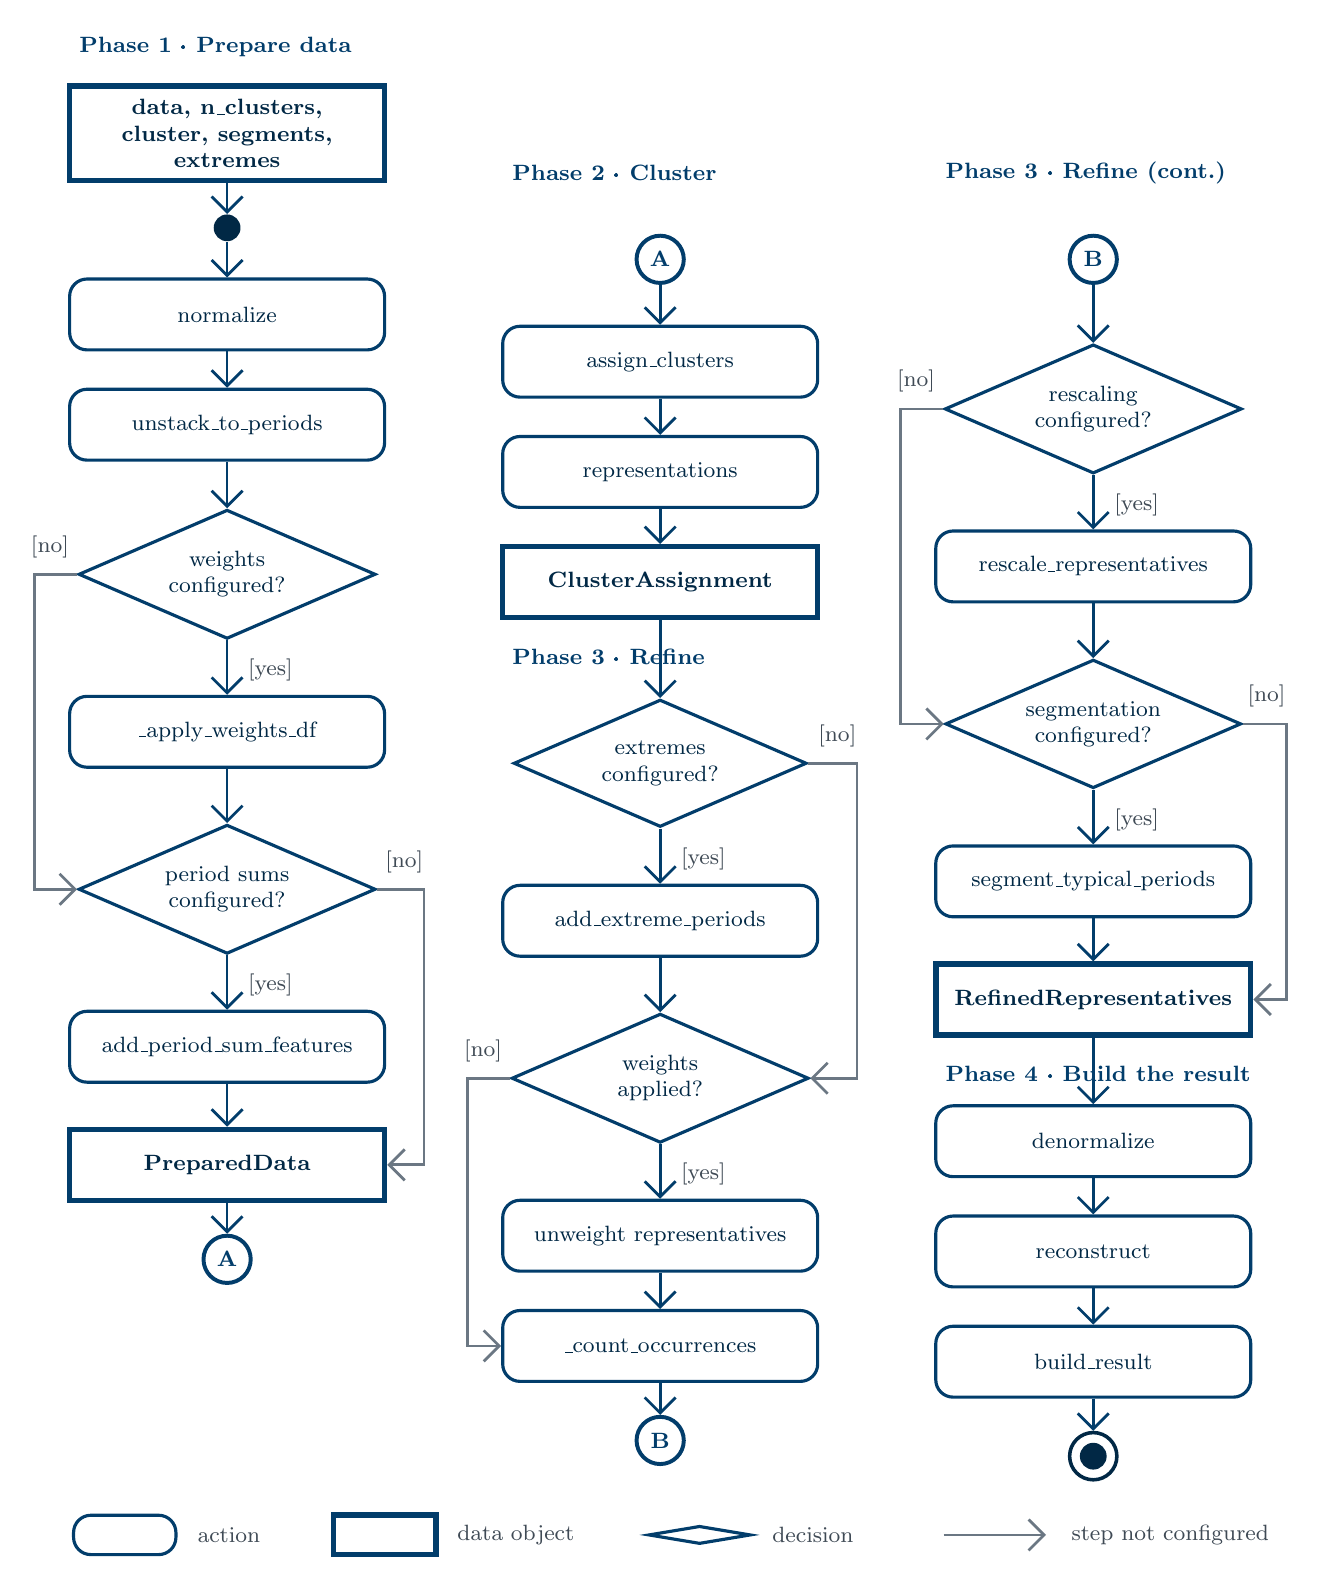
\begin{tikzpicture}[
  x=1mm, y=1mm,
  % UML action node — rounded rectangle
  act/.style={
    draw=fzjblue, line width=0.4mm, fill=white, text=fzjdark, rounded corners=2.2mm,
    minimum width=40mm, minimum height=9mm, align=center, font=\footnotesize},
  % UML object node — sharp corners and a heavier rule, so it never reads as an action
  obj/.style={
    draw=fzjblue, line width=0.7mm, fill=white, text=fzjdark,
    minimum width=40mm, minimum height=9mm, align=center, font=\footnotesize\bfseries},
  % aspect 2.3 with text width 21 mm makes the diamond exactly 40 mm wide and
  % 17.4 mm tall, so it occupies the same lane as an action box. Every guard is
  % broken by hand into two lines: a third line would widen it past the column.
  dec/.style={
    diamond, aspect=2.3, draw=fzjblue, line width=0.4mm, fill=white, text=fzjdark,
    inner sep=0.5mm, text width=21mm, align=center, font=\footnotesize},
  % activity parameter node: what the caller constructs and hands to aggregate()
  objp/.style={
    draw=fzjblue, line width=0.7mm, fill=white, text=fzjdark,
    minimum width=40mm, minimum height=12mm, align=center, font=\footnotesize\bfseries},
  % UML connector node: the lettered circle that continues a flow elsewhere
  conn/.style={
    circle, draw=fzjblue, line width=0.5mm, fill=white, text=fzjblue,
    minimum size=6mm, inner sep=0, font=\footnotesize\bfseries},
  flow/.style={-{Straight Barb[scale=1.6]}, draw=fzjblue, line width=0.35mm},
  skip/.style={-{Straight Barb[scale=1.6]}, draw=skipgrey, line width=0.35mm},
  g/.style={font=\footnotesize, text=greytext, inner sep=1.2pt},
  phase/.style={font=\footnotesize\bfseries, text=fzjblue, anchor=west},
  lgd/.style={font=\footnotesize, text=greytext, anchor=west}
]
% no hyphenation: a broken "extreme peri-ods" inside a diamond reads badly
\hyphenpenalty=10000 \exhyphenpenalty=10000

% ══ Column 1 — Phase 1, Prepare data ════════════════════════════════════
\node[phase] at (5,23) {Phase 1 \textperiodcentered{} Prepare data};
\node[objp] (params) at (25,12)
  {data, n\_clusters,\\ cluster, segments,\\ extremes};
\node[circle, fill=fzjdark, minimum size=3.4mm, inner sep=0] (start) at (25,0) {};
\node[act]  (n1) at (25,-11)  {normalize};
\node[act]  (n2) at (25,-25)  {unstack\_to\_periods};
\node[dec]  (d1) at (25,-44)  {weights\\configured?};
\node[act]  (n3) at (25,-64)  {\_apply\_weights\_df};
\node[dec]  (d2) at (25,-84)  {period sums\\configured?};
\node[act]  (n4) at (25,-104) {add\_period\_sum\_features};
\node[obj]  (o1) at (25,-119) {PreparedData};
\node[conn] (ca) at (25,-131) {A};

\draw[flow] (params) -- (start);
\draw[flow] (start) -- (n1);
\draw[flow] (n1) -- (n2);
\draw[flow] (n2) -- (d1);
\draw[flow] (d1) -- (n3);
\draw[flow] (n3) -- (d2);
\draw[flow] (d2) -- (n4);
\draw[flow] (n4) -- (o1);
\draw[flow] (o1) -- (ca);
\draw[skip] (d1.west) -- (0.5,-44) -- (0.5,-84) -- (d2.west);
\draw[skip] (d2.east) -- (50,-84) -- (50,-119) -- (o1.east);

\node[g] at (30.5,-56.2) {[yes]};
\node[g] at (30.5,-96.2) {[yes]};
\node[g] at (2.5,-40.5)  {[no]};
\node[g] at (47.5,-80.5) {[no]};

% ══ Column 2 — Phase 2, then the first half of Phase 3 ══════════════════
\node[phase] at (60,7) {Phase 2 \textperiodcentered{} Cluster};
\node[conn] (cb) at (80,-4) {A};
% two steps, per cluster_and_represent's own docstring: assign_clusters puts each
% period in a cluster, then representations derives the representative profile
\node[act]  (n5) at (80,-17)  {assign\_clusters};
\node[act]  (n6) at (80,-31)  {representations};
\node[obj]  (o2) at (80,-45)  {ClusterAssignment};
\node[phase] at (60,-54.5) {Phase 3 \textperiodcentered{} Refine};
\node[dec]  (d3) at (80,-68)  {extremes\\configured?};
\node[act]  (m1) at (80,-88)  {add\_extreme\_periods};
% inline in refine_representatives: representatives are divided back through the
% weight vector before rescale and denormalize, which expect unweighted data
\node[dec]  (d6) at (80,-108) {weights\\applied?};
\node[act]  (m2) at (80,-128) {unweight representatives};
\node[act]  (m3) at (80,-142) {\_count\_occurrences};
\node[conn] (cc) at (80,-154) {B};

\draw[flow] (cb) -- (n5);
\draw[flow] (n5) -- (n6);
\draw[flow] (n6) -- (o2);
\draw[flow] (o2) -- (d3);
\draw[flow] (d3) -- (m1);
\draw[flow] (m1) -- (d6);
\draw[flow] (d6) -- (m2);
\draw[flow] (m2) -- (m3);
\draw[flow] (m3) -- (cc);
\draw[skip] (d3.east) -- (105,-68) -- (105,-108) -- (d6.east);
\draw[skip] (d6.west) -- (55.5,-108) -- (55.5,-142) -- (m3.west);

\node[g] at (85.5,-80.2)  {[yes]};
\node[g] at (85.5,-120.2) {[yes]};
\node[g] at (102.5,-64.5) {[no]};
\node[g] at (57.5,-104.5) {[no]};

% ══ Column 3 — rest of Phase 3, then Phase 4 ════════════════════════════
\node[phase] at (115,7) {Phase 3 \textperiodcentered{} Refine (cont.)};
\node[conn] (cd) at (135,-4)  {B};
\node[dec]  (d4) at (135,-23) {rescaling\\configured?};
\node[act]  (m4) at (135,-43) {rescale\_representatives};
\node[dec]  (d5) at (135,-63) {segmentation\\configured?};
\node[act]  (m5) at (135,-83) {segment\_typical\_periods};
\node[obj]  (o3) at (135,-98) {RefinedRepresentatives};
\node[phase] at (115,-107.5) {Phase 4 \textperiodcentered{} Build the result};
\node[act]  (m6) at (135,-116) {denormalize};
\node[act]  (m7) at (135,-130) {reconstruct};
\node[act]  (m8) at (135,-144) {build\_result};
\node[circle, draw=fzjdark, line width=0.45mm, fill=white, minimum size=6mm, inner sep=0]
  (finish) at (135,-156) {};
\fill[fzjdark] (finish) circle (1.7mm);

\draw[flow] (cd) -- (d4);
\draw[flow] (d4) -- (m4);
\draw[flow] (m4) -- (d5);
\draw[flow] (d5) -- (m5);
\draw[flow] (m5) -- (o3);
\draw[flow] (o3) -- (m6);
\draw[flow] (m6) -- (m7);
\draw[flow] (m7) -- (m8);
\draw[flow] (m8) -- (finish);
\draw[skip] (d4.west) -- (110.5,-23) -- (110.5,-63) -- (d5.west);
\draw[skip] (d5.east) -- (159.5,-63) -- (159.5,-98) -- (o3.east);

\node[g] at (140.5,-35.2) {[yes]};
\node[g] at (140.5,-75.2) {[yes]};
\node[g] at (112.5,-19.5) {[no]};
\node[g] at (157,-59.5)   {[no]};

% ══ shape key ═══════════════════════════════════════════════════════════
% One row across the bottom, BELOW every column (the deepest thing above it is
% column 3's final node at y -159). A two-by-two block tucked into column 1's
% free space was tried first and does not work: its right-hand labels reach
% x = 77, which is inside column 2, where _count_occurrences and the B
% connector still sit at y -142 and y -154.
\node[act, minimum width=13mm, minimum height=5mm, font=\tiny] at (12,-166) {};
\node[lgd] at (20,-166) {action};
\node[obj, minimum width=13mm, minimum height=5mm, font=\tiny] at (45,-166) {};
\node[lgd] at (53,-166) {data object};
\node[dec, minimum width=13mm, text width=6mm, aspect=2.6, inner sep=0] at (85,-166) {};
\node[lgd] at (93,-166) {decision};
\draw[skip] (116,-166) -- (129,-166);
\node[lgd] at (131,-166) {step not configured};

\end{tikzpicture}
\end{document}
